% !TEX root = ../../main.tex

\section{Calorimetry MIL-127(Fe)}

\begin{figure}[htb]
    \centering

    \begin{subfigure}{0.19\linewidth}
        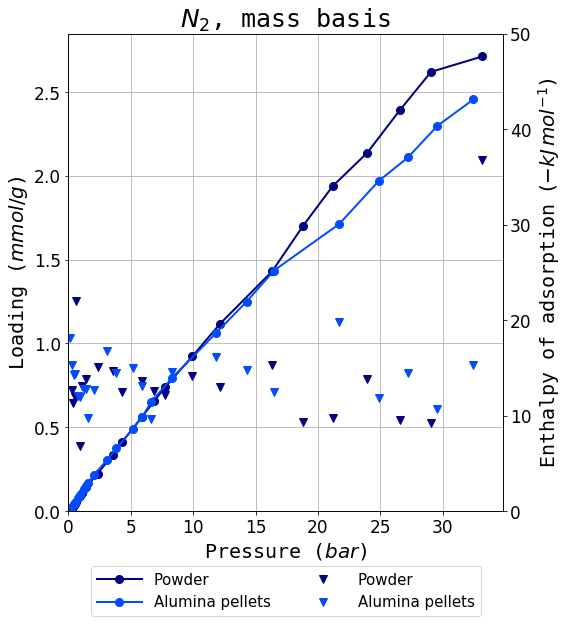
\includegraphics[width=\textwidth]{calo/MIL-127(Fe)/N2-mass-basis-iso}%
        \label{fgr:mil127n2mass}
    \end{subfigure}
    \begin{subfigure}{0.19\linewidth}
        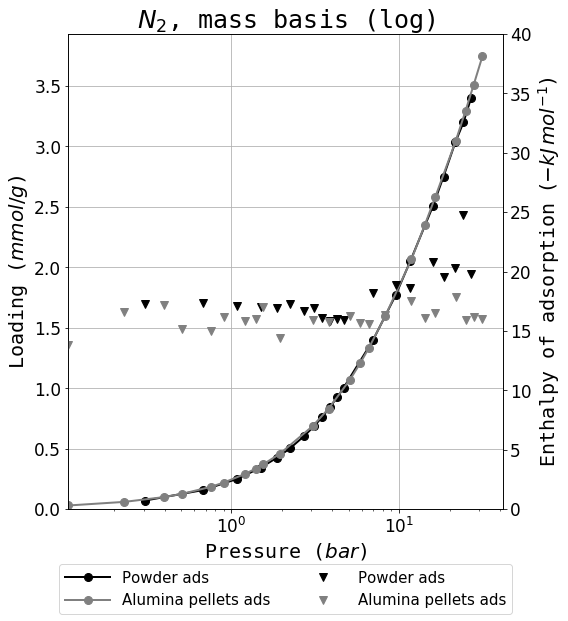
\includegraphics[width=\textwidth]{calo/MIL-127(Fe)/N2-mass-basis-log-iso}%
        \label{fgr:mil127n2masslog}
    \end{subfigure}
    \begin{subfigure}{0.19\linewidth}
        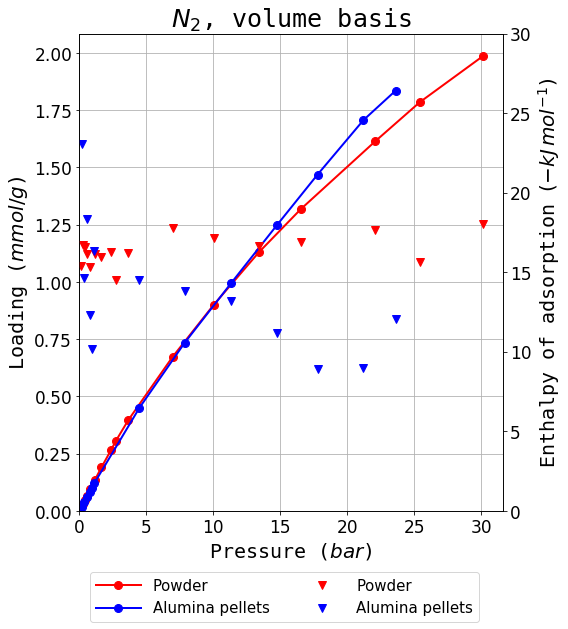
\includegraphics[width=\textwidth]{calo/MIL-127(Fe)/N2-volume-basis-iso}%
        \label{fgr:mil127n2volume}
    \end{subfigure}
    \begin{subfigure}{0.19\linewidth}
        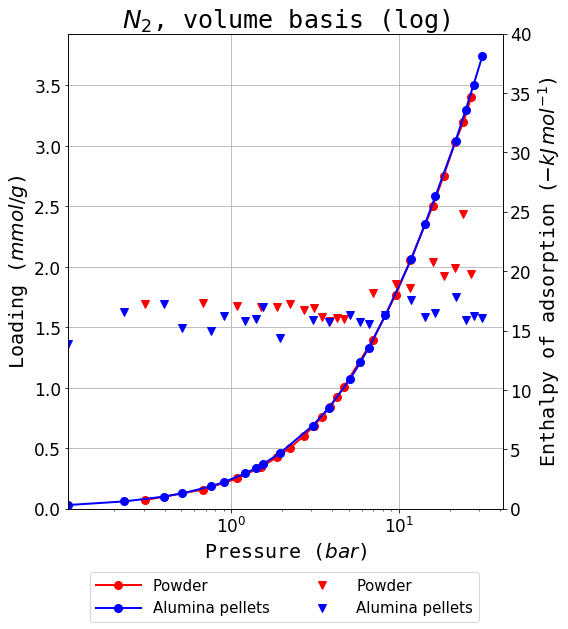
\includegraphics[width=\textwidth]{calo/MIL-127(Fe)/N2-volume-basis-log-iso}%
        \label{fgr:mil127n2volumelog}
    \end{subfigure}
    \begin{subfigure}{0.19\linewidth}
        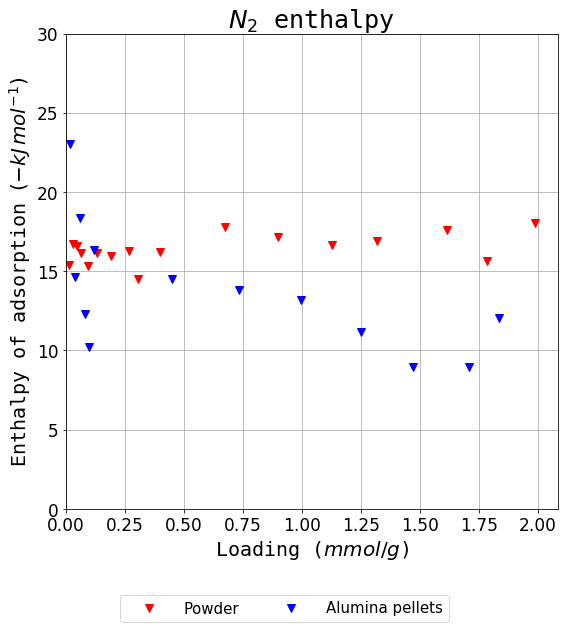
\includegraphics[width=\textwidth]{calo/MIL-127(Fe)/N2-enth}%
        \label{fgr:mil127n2enth}
    \end{subfigure}
    

    \begin{subfigure}{0.19\textwidth}
        \includegraphics[width=\textwidth]{calo/MIL-127(Fe)/co2-mass-basis-iso}%
        \label{fgr:mil127co2mass}
    \end{subfigure}
    \begin{subfigure}{0.19\textwidth}
        \includegraphics[width=\textwidth]{calo/MIL-127(Fe)/co2-mass-basis-log-iso}%
        \label{fgr:mil127co2masslog}
    \end{subfigure}
    \begin{subfigure}{0.19\textwidth}
        \includegraphics[width=\textwidth]{calo/MIL-127(Fe)/co2-volume-basis-iso}%
        \label{fgr:mil127co2volume}
    \end{subfigure}
    \begin{subfigure}{0.19\textwidth}
        \includegraphics[width=\textwidth]{calo/MIL-127(Fe)/co2-volume-basis-log-iso}%
        \label{fgr:mil127co2volumelog}
    \end{subfigure}
    \begin{subfigure}{0.19\textwidth}
        \includegraphics[width=\textwidth]{calo/MIL-127(Fe)/co2-enth}%
        \label{fgr:mil127co2enth}
    \end{subfigure}


    \begin{subfigure}{0.19\textwidth}
        \includegraphics[width=\textwidth]{calo/MIL-127(Fe)/co-mass-basis-iso}%
        \label{fgr:mil127comass}
    \end{subfigure}
    \begin{subfigure}{0.19\textwidth}
        \includegraphics[width=\textwidth]{calo/MIL-127(Fe)/co-mass-basis-log-iso}%
        \label{fgr:mil127comasslog}
    \end{subfigure}
    \begin{subfigure}{0.19\textwidth}
        \includegraphics[width=\textwidth]{calo/MIL-127(Fe)/co-volume-basis-iso}%
        \label{fgr:mil127covolume}
    \end{subfigure}
    \begin{subfigure}{0.19\textwidth}
        \includegraphics[width=\textwidth]{calo/MIL-127(Fe)/co-volume-basis-log-iso}%
        \label{fgr:mil127covolumelog}
    \end{subfigure}
    \begin{subfigure}{0.19\textwidth}
        \includegraphics[width=\textwidth]{calo/MIL-127(Fe)/co-enth}%
        \label{fgr:mil127coenth}
    \end{subfigure}


    \begin{subfigure}{0.19\textwidth}
        \includegraphics[width=\textwidth]{calo/MIL-127(Fe)/ch4-mass-basis-iso}%
        \label{fgr:mil127ch4mass}
    \end{subfigure}
    \begin{subfigure}{0.19\textwidth}
        \includegraphics[width=\textwidth]{calo/MIL-127(Fe)/ch4-mass-basis-log-iso}%
        \label{fgr:mil127ch4masslog}
    \end{subfigure}
    \begin{subfigure}{0.19\textwidth}
        \includegraphics[width=\textwidth]{calo/MIL-127(Fe)/ch4-volume-basis-iso}%
        \label{fgr:mil127ch4volume}
    \end{subfigure}
    \begin{subfigure}{0.19\textwidth}
        \includegraphics[width=\textwidth]{calo/MIL-127(Fe)/ch4-volume-basis-log-iso}%
        \label{fgr:mil127ch4volumelog}
    \end{subfigure}
    \begin{subfigure}{0.19\textwidth}
        \includegraphics[width=\textwidth]{calo/MIL-127(Fe)/ch4-enth}%
        \label{fgr:mil127ch4enth}
    \end{subfigure}

    \caption{Complete isotherm and enthalpy dataset for MIL-127(Fe)}
    
\end{figure}
\begin{figure}[htb]\ContinuedFloat%

    \begin{subfigure}{0.19\textwidth}
        \includegraphics[width=\textwidth]{calo/MIL-127(Fe)/c2h6-mass-basis-iso}%
        \label{fgr:mil127c2h6mass}
    \end{subfigure}
    \begin{subfigure}{0.19\textwidth}
        \includegraphics[width=\textwidth]{calo/MIL-127(Fe)/c2h6-mass-basis-log-iso}%
        \label{fgr:mil127c2h6masslog}
    \end{subfigure}
    \begin{subfigure}{0.19\textwidth}
        \includegraphics[width=\textwidth]{calo/MIL-127(Fe)/c2h6-volume-basis-iso}%
        \label{fgr:mil127c2h6volume}
    \end{subfigure}
    \begin{subfigure}{0.19\textwidth}
        \includegraphics[width=\textwidth]{calo/MIL-127(Fe)/c2h6-volume-basis-log-iso}%
        \label{fgr:mil127c2h6volumelog}
    \end{subfigure}
    \begin{subfigure}{0.19\textwidth}
        \includegraphics[width=\textwidth]{calo/MIL-127(Fe)/c2h6-enth}%
        \label{fgr:mil127c2h6enth}
    \end{subfigure}


    \begin{subfigure}{0.19\textwidth}
        \includegraphics[width=\textwidth]{calo/MIL-127(Fe)/c3h8-mass-basis-iso}%
        \label{fgr:mil127c3h8mass}
    \end{subfigure}
    \begin{subfigure}{0.19\textwidth}
        \includegraphics[width=\textwidth]{calo/MIL-127(Fe)/c3h8-mass-basis-log-iso}%
        \label{fgr:mil127c3h8masslog}
    \end{subfigure}
    \begin{subfigure}{0.19\textwidth}
        \includegraphics[width=\textwidth]{calo/MIL-127(Fe)/c3h8-volume-basis-iso}%
        \label{fgr:mil127c3h8volume}
    \end{subfigure}
    \begin{subfigure}{0.19\textwidth}
        \includegraphics[width=\textwidth]{calo/MIL-127(Fe)/c3h8-volume-basis-log-iso}%
        \label{fgr:mil127c3h8volumelog}
    \end{subfigure}
    \begin{subfigure}{0.19\textwidth}
        \includegraphics[width=\textwidth]{calo/MIL-127(Fe)/c3h8-enth}%
        \label{fgr:mil127c3h8enth}
    \end{subfigure}

    \begin{subfigure}{0.19\textwidth}
        \includegraphics[width=\textwidth]{calo/MIL-127(Fe)/c3h6-mass-basis-iso}%
        \label{fgr:mil127c3h6mass}
    \end{subfigure}
    \begin{subfigure}{0.19\textwidth}
        \includegraphics[width=\textwidth]{calo/MIL-127(Fe)/c3h6-mass-basis-log-iso}%
        \label{fgr:mil127c3h6masslog}
    \end{subfigure}
    \begin{subfigure}{0.19\textwidth}
        \includegraphics[width=\textwidth]{calo/MIL-127(Fe)/c3h6-volume-basis-iso}%
        \label{fgr:mil127c3h6volume}
    \end{subfigure}
    \begin{subfigure}{0.19\textwidth}
        \includegraphics[width=\textwidth]{calo/MIL-127(Fe)/c3h6-volume-basis-log-iso}%
        \label{fgr:mil127c3h6volumelog}
    \end{subfigure}
    \begin{subfigure}{0.19\textwidth}
        \includegraphics[width=\textwidth]{calo/MIL-127(Fe)/c3h6-enth}%
        \label{fgr:mil127c3h6enth}
    \end{subfigure}


    \begin{subfigure}{0.19\textwidth}
        \includegraphics[width=\textwidth]{calo/MIL-127(Fe)/c4h10-mass-basis-iso}%
        \label{fgr:mil127c4h10mass}
    \end{subfigure}
    \begin{subfigure}{0.19\textwidth}
        \includegraphics[width=\textwidth]{calo/MIL-127(Fe)/c4h10-mass-basis-log-iso}%
        \label{fgr:mil127c4h10masslog}
    \end{subfigure}
    \begin{subfigure}{0.19\textwidth}
        \includegraphics[width=\textwidth]{calo/MIL-127(Fe)/c4h10-volume-basis-iso}%
        \label{fgr:mil127c4h10volume}
    \end{subfigure}
    \begin{subfigure}{0.19\textwidth}
        \includegraphics[width=\textwidth]{calo/MIL-127(Fe)/c4h10-volume-basis-log-iso}%
        \label{fgr:mil127c4h10volumelog}
    \end{subfigure}
    \begin{subfigure}{0.19\textwidth}
        \includegraphics[width=\textwidth]{calo/MIL-127(Fe)/c4h10-enth}%
        \label{fgr:mil127c4h10enth}
    \end{subfigure}

    \caption{Complete isotherm and enthalpy dataset for MIL-127(Fe)}%
    \label{fgr:calomil127}
\end{figure}
